\documentclass[a4paper]{article}

\usepackage[ngerman]{babel}
\usepackage[utf8]{inputenc}
\usepackage{amsmath}
\usepackage{amssymb}
\usepackage{amsthm}
\usepackage{booktabs}
\usepackage{array}
\usepackage{tabularx}
\usepackage{color}
\usepackage{ulem}
\usepackage{fancyhdr}
\usepackage{graphicx}
\usepackage{geometry}
\usepackage{polynom}
\usepackage{pgf,tikz}
\usepackage{amsfonts}
\usepackage{cancel}
\usepackage{mathcomp}
\usepackage{mathrsfs}
\usepackage{multirow}
\usepackage{dsfont}
\usepackage{
    amscd,
    amsfonts,
    amsmath,
    amssymb,
    amsthm,
}
\usepackage{tikz}
\usepackage{stmaryrd}
\usepackage{ulsy}

\newcommand{\IR}{\mathbb{R}}

\usetikzlibrary{trees,decorations,arrows,automata,shadows,positioning,plotmarks}
\geometry{left=2cm, top=1.5cm, right=2cm, bottom=2cm}

\parindent0pt

\begin{document}

  \begin{flushright}
    \today
  \end{flushright}
  \begin{center}
    \Large\textbf{{GKI - Hausaufgaben 2}}\\
  \end{center}

  \begin{center}
        \large\textsl{Tao Xu, 343390 - Mitja Richter, 324680 - Björn Kapelle, 320438 - Marcus Weber, 320402}\\
  \end{center}


\section*{Aufgabe 2}
\subsection*{2.a)}
Der gegebene Tabelle sieht wie folgt aus.\\

\begin{tabular}{|cc|cc|cc|cc|}
\hline
\textbf{1} &  & 1 & 2 & 1 & 2 & 1 & 2\\
  &  & 3 & 4 & 3 & 4 & 3 & 4\\
\hline
 & \textbf{2} & 1 & 2 & 1 & 2 & 1 & 2\\
  &  & 3 & 4 & 3 & 4 & 3 & 4\\
\hline
1 & 2 & 1 & 2 & 1 & 2 &  & \\
 3 & 4 & 3 & 4 & 3 & 4 & \textbf{3} & \\
\hline
1 & 2 & 1 & 2 & 1 & 2 & 1 & 2\\
 3 & 4 & 3 & 4 & 3 & 4 & 3 & 4\\
\hline
\end{tabular} \\
\\
Aus dieser Tabelle entfernen wir nun Elemente durch die beiden Constraints \\
$\forall i,j,k \in \{ 1, \ldots ,n\}$ mit $j \ne k: M(i,j) \ne M(i,k)$ (rot gef\"arbt) und \\
$\forall i,j,k \in \{ 1, \ldots ,n\}$ mit $j \ne k: M(j,i) \ne M(k,i)$ (blau gef\"arbt).\\
Das hei\ss t folgende Tabelle entsteht:\\

\begin{tabular}{|cc|cc|cc|cc|}
\hline
\textbf{1} &  & \textcolor{red}{\sout{1}} & 2 & \textcolor{red}{\sout{1}} & 2 & \textcolor{red}{\sout{1}} & 2\\
  &  & 3 & 4 & 3 & 4 & \textcolor{blue}{\sout{3}} & 4\\
\hline
 & \textbf{2} & 1 & \textcolor{red}{\sout{2}} & 1 & \textcolor{red}{\sout{2}} & 1 & \textcolor{red}{\sout{2}}\\
  &  & 3 & 4 & 3 & 4 & \textcolor{blue}{\sout{3}} & 4\\
\hline
\textcolor{blue}{\sout{1}} & \textcolor{blue}{\sout{2}} & 1 & 2 & 1 & 2 &  & \\
 \textcolor{red}{\sout{3}} & 4 & \textcolor{red}{\sout{3}} & 4 & \textcolor{red}{\sout{3}} & 4 & \textbf{3} & \\
\hline
\textcolor{blue}{\sout{1}} & \textcolor{blue}{\sout{2}} & 1 & 2 & 1 & 2 & 1 & 2\\
 3 & 4 & 3 & 4 & 3 & 4 & \textcolor{blue}{\sout{3}} & 4\\
\hline
\end{tabular} \\

\subsection*{2.b)}
Unsere Heuristik ist: w\"ahle Variable mit den wenigsten konsistenten Werten. Gibt es mehrere, die diese Bedingung erf\"ullen, so betrachtet man die Variable die die geringste Zeilennummer hat. Sollten auch hier mehrere m\"oglich sein, so betrachtet man diesen Variablen, die mit der kleinsten Spaltennummer. (sp\"atestens diese ist eindeutig)\\
Wenn wir dies auf unser Problem anwenden wird $M(2,1)$ (man beachte, dass die Zeilen von unten nach oben und die Spalten von links nach rechts durchnummeriert sind) als erstes gew\"ahlt. Wir nehmen diese Heuristik, weil dadurch weniger Zweige erzeugt werden. Zudem wird schneller herausgefunden, ob die Belegung zu einer g\"ultigen  L\"osung f\"uhren kann, als wenn man durch Betrachtung der anderen Variablen, die auf dieses Element durch ein Constraint Einfluss haben, L\"osungen ausschlie\ss en m\"ochte. 
Andernfalls m\"usste man die anderen Variablen betrachten, die auf dieses Element Einfluss nehmen k\"onnen, und diese durch mehr verschiedene F\"alle zu einer Einschr\"ankung f\"uhren. \\

\subsection*{2.c)}
Nach unserer Heuristik betrachten wir zun\"achst $M(2,1)$. Dort ist lediglich der Eintrag $4$ noch möglich. Daraus ergibt sich folgende Tabelle:\\

\begin{tabular}{|cc|cc|cc|cc|}
\hline
\textbf{1}& & & 2 & & 2 & & 2\\
  & & 3 & 4 & 3 & 4 & & 4\\
\hline
 & \textbf{2} & 1 &  & 1 &  & 1 & \\
  &  & 3 & 4 & 3 & 4 &  & 4\\
\hline
&  & 1 & 2 & 1 & 2 &  & \\
  & \textbf{4} & & \textcolor{red}{\sout{4}} & & \textcolor{red}{\sout{4}} & \textbf{3} & \\
\hline
 &  & 1 & 2 & 1 & 2 & 1 & 2\\
 3 & \textcolor{blue}{\sout{4}} & 3 & 4 & 3 & 4 &  & 4\\
\hline
\end{tabular} \\
\\
Damit ergeben sich folgende neue Wertebereiche: \\
$M(1,1) \in \{ 3 \}$, $M(2,2) \in \{ 1,2 \}$ und $M(2,3) \in \{1,2\}$.


\section*{Aufgabe 3}
\subsection*{3.a) und b) und d)}
Der bewertete Suchbaum mit Cut-Offs sieht folgenderma{\ss}en aus:

\begin{figure}[h]
\centering
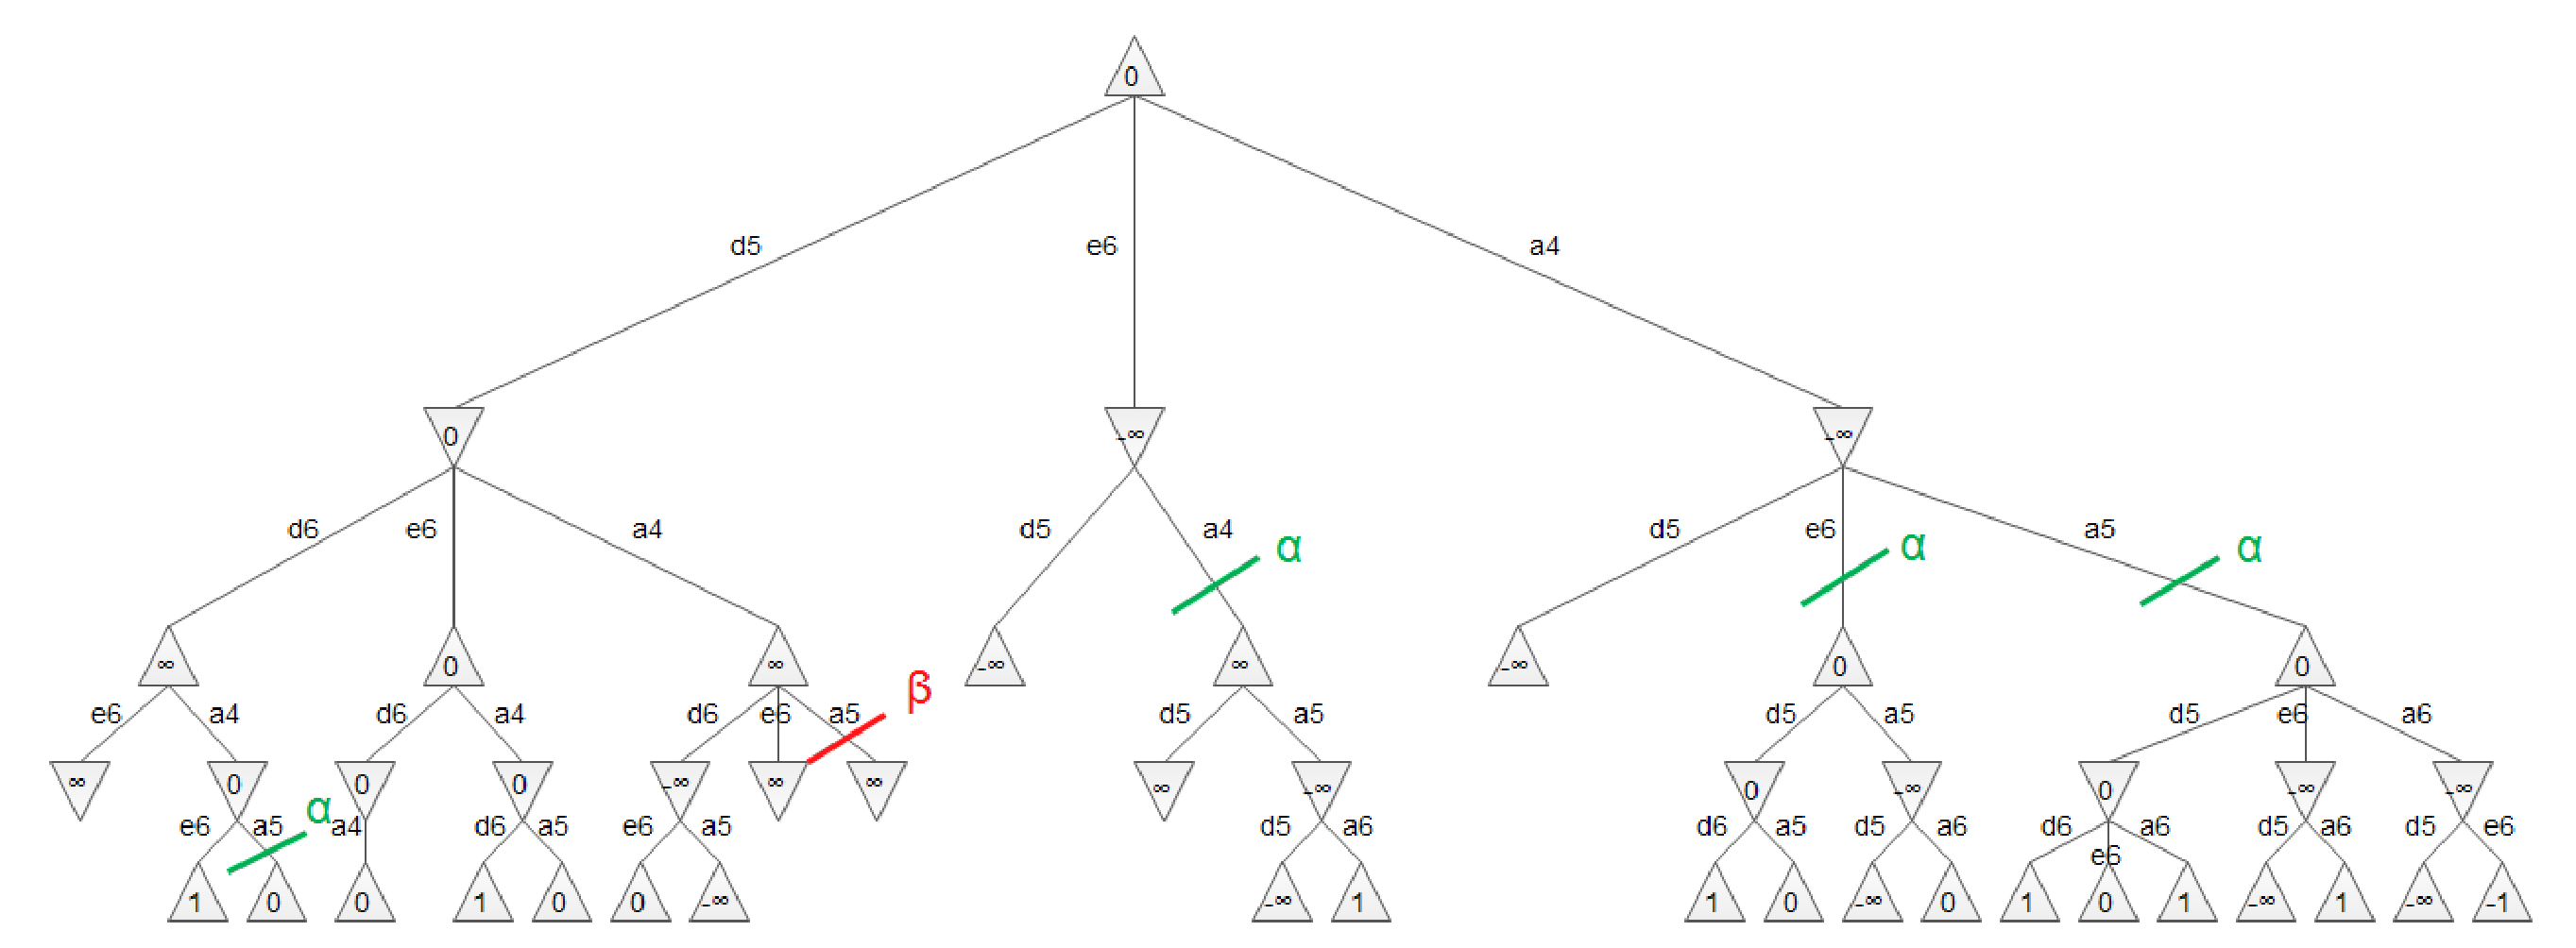
\includegraphics[width=\columnwidth]{blatt2aufgabe3}
\end{figure}

\subsection*{3.c)}
Der Horizonteffekt tritt auf, wenn die Tiefensuche bei einer bestimmten Baumtiefe (hier: $d=4$) abgebrochen wird. Da der Agent somit unterhalb dieser Tiefe v\"ollig blind ist, kann es sein, dass Blattknoten anders bewertet werden, als wenn man die tieferen Ebenen auch ber\"ucksichtigen w\"urde.\\
\\
Ein Beispiel daf\"ur ist in unserem Fall der Spielverlauf $d5 - e6 - d6 - a4$. Dieses Blatt ist nur mit $0$ bewertet, da sowohl gelb als auch rot einen offenen Dreier haben. W\"are die Suchtiefe aber gr\"o{\ss}er, w\"usste MAX nat\"urlich, dass er im n\"achsten Zug gewinnt und w\"urde entsprechend den Knoten mit $\infty$ bewerten. Damit h\"atte MAX dann eine sichere Gewinnstrategie.

\end{document}
